\documentclass[11pt]{report}
\usepackage{geometry}                % See geometry.pdf to learn the layout options. There are lots.
\geometry{letterpaper}                   % ... or a4paper or a5paper or ... 
%\geometry{landscape}                % Activate for for rotated page geometry
%\usepackage[parfill]{parskip}    % Activate to begin paragraphs with an empty line rather than an indent

% Custom doxygen styles, packaged as an envronment instead
\usepackage{mydoxygen}

\usepackage{pdfpages}
\usepackage{graphicx}
\usepackage{float}
\usepackage{amssymb}
\usepackage{todonotes}
\usepackage{epstopdf}
\usepackage{hyperref}
\usepackage{wrapfig}
\usepackage{siunitx}
\usepackage[version=3]{mhchem} % For chemical typesetting
\usepackage[toc,page]{appendix}
\usepackage{booktabs}
\DeclareGraphicsRule{.tif}{png}{.png}{`convert #1 `dirname #1`/`basename #1 .tif`.png}

% Make subtitle
\usepackage{titling}
\newcommand{\subtitle}[1]{%
  \posttitle{%
    \par\end{center}
    \begin{center}\textit{\large#1}\end{center}
    \vskip0.5em}%
}

\graphicspath{{images/}}

% Define numbers
\newcommand{\baudrate}{57600}
\newcommand{\VExcite}{1.0}
\newcommand{\RGain}{\SI{51}{\kilo\ohm}}
\newcommand{\RSeries}{\SI{1}{\kilo\ohm}}
\newcommand{\RSet}{\SI{10}{\kilo\ohm}}
\newcommand{\tempRange}{\SI{7}{\celsius} to \SI{36}{\celsius}}

\newcommand{\tempCtrlVer}{v4.3D}

\title{Digital isolated 4 channel temperature controller}
\subtitle{Version: \tempCtrlVer}
\author{Charles Baynham}
\date{\today}                                           % Activate to display a given date or no date

\setlength{\parskip}{4mm plus 4mm minus 2mm}

% Call chapters "sections"
\renewcommand{\chaptername}{Section}

\begin{document}
\maketitle

\tableofcontents
\clearpage

\chapter{Overview} % (fold)
\label{sec:overview}

\begin{figure}[h]
	\centering
	\includegraphics[width=0.65\textwidth]{BoardRender}
	\caption{Picture / render of the board}
	\label{fig:wholeboard}
\end{figure}

This manual describes the operation and design processes behind the \ce{Yb+} digital temperature controller, version~\tempCtrlVer. The controller is designed for taking high precision temperature measurements via a thermistor and applying low bandwidth PID feedback in response.

\section{Microprocessor}

The device is controlled by an on-board microprocessor running at \SI{16}{MHz}. It operates in headless mode and can be configured to automatically recover from power failures. Setup and monitoring is by USB connection, baud rate 57600. This USB connection is electrically isolated from the rest of the board to prevent ground loops or digital noise. 

\section{Output}

Output is by either OPA458 high power opamps. Output can be up to \SI{1}{\A} continuous (see Figure~\ref{fig:OPA_SOA}), at voltages up to \SI{24}{\volt} depending on the power supply, $V_S$. 

The board contains space for four output channels allowing for voltages between \SI{0}{\volt} and $V_S$. Alternatively the channels can be combined to form two bipolar output channels, permitting outputs up to $\pm V_S$. See Section~\ref{sec:connector_pins} for details. Note that these are not rail-to-rail opamps: the minimum possible output is around \SI{300}{\milli\volt}, so applications that require lower voltages than these must use the bipolar configuration. 

\section{Input}

Error signal acquisition is done by taking a balanced measurement between a thermistor and a set resistor. The board produces an excitation voltage, usually \SI{\VExcite}{\volt}, and measures the difference in current between the thermistor and resistor to produce a temperature measurement. For less demanding applications the set resistor can be on-board. For the highest stability, the precision resistor should be placed next to its paired thermistor. 

This measurement is performed by an INA330 chip, of which there are two present on the board. The entire analogue section is electrically isolated from the rest of the board to prevent noise on the electrical ground affecting the measurement. 

There are therefore two possible input channels by balanced thermistor measurements. See Section~\ref{sec:connector_pins} for details. 

\section{Commands}

Control of the device is via serial connection over USB. It accepts commands, detailed in Appendix~\ref{chap:available_commands}. A Labview interface is also available which handles this communication. 

\chapter{Connector Pins} % (fold)
\label{sec:connector_pins}

This section describes the usage and pin-out for all the connectors on the board. See Figure~\ref{fig:connectors} for reference as to their locations. 

\begin{figure}[h!]
	\centering
	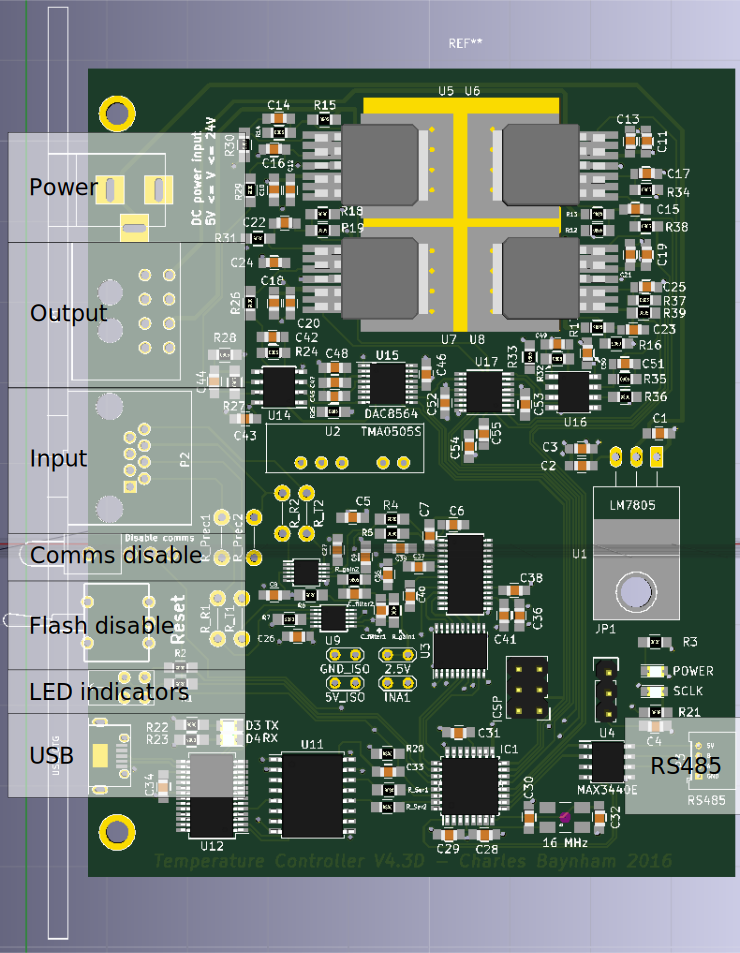
\includegraphics[width=0.5\textwidth]{BoardLabelled/Labelled}
	\caption{Layout of connectors on the board}
	\label{fig:connectors}
\end{figure}

\section{Power}

Power supply is via a standard \SI{2.1}{mm}, centre-positive barrel connector. The board expects a DC voltage up to \SI{30}{\volt} and of at least \SI{7}{\volt}, limited by the LM7805 power regulator that powers most of the electronics. Whatever voltage is supplied here will be the maximum possible output control voltage. When choosing what voltage to supply, the user should take note of considerations in Section~\ref{sub:opa_choice} regarding opamp overheating. 

\section{Output}

\begin{table}[H]
	
	\centering

	\begin{tabular}{ll}
	\toprule
	Pin & Purpose  \\ \midrule
	1   & GND      \\
	2   & GND      \\
	3   & GND      \\
	4   & GND      \\
	5   & Unipolar output 1 or bipolar 1 positive output ({\tt BPA}) \\
	6   & Unipolar output 2 or bipolar 1 negative output ({\tt BPA}) \\
	7   & Unipolar output 3 or bipolar 2 positive output ({\tt BPB}) \\
	8   & Unipolar output 4 or bipolar 2 negative output ({\tt BPB}) \\ \bottomrule
	\end{tabular}

	\caption{Pin connections for the output}
	\label{tab:output_pins}

\end{table}

\begin{wrapfigure}{l}{0.3\textwidth}
\centering
\includegraphics[width=0.25\textwidth]{MicroFit/MicroFit_labelled}
\caption{Molex MICRO FIT 3.0 series 43045 output connector}
\end{wrapfigure}

The output connector is a Molex MICRO\_FIT 3.0 series 43045. It has 8 contacts, 4 of which are the OPA outputs and 4 are GND. In unipolar operation the device to be controlled (hereafter the plant) should be connected to one of the channels and GND. For bipolar operation connect to both the OPA output channels and leave the GND pins unconnected. 

\clearpage
\section{Thermistor input}

\begin{wrapfigure}{l}{0.3\textwidth}
\centering
\includegraphics[width=0.2\textwidth]{RJ45-Pinout-T568B}
\caption[Pinout for a RJ45 T568-B connector]{Pinout for a RJ45 T568-B connector \protect\footnotemark}
\end{wrapfigure}

\footnotetext{Image from \url{http://blog.showmecables.com/rj45-pinout/}}

\begin{table}[H]
	
	\centering

	\begin{tabular}{rll}
	\toprule
	Pin & Common colour & Purpose  \\ \midrule
	1   & Orange and white & GND      \\
	2   & Orange & Set resistor 1 +      \\
	3   & Green and white & GND	   \\
	4   & Blue & Thermistor 1 + 	   \\ 
	5   & Blue and white & GND      \\
	6   & Green & Set resistor 2 +      \\
	7   & Brown and white & GND      \\
	8   & Brown & Thermistor 2 +      \\
	\bottomrule
	\end{tabular}

	\caption{Pin connections for the error signal input}
	\label{tab:input_pins}

\end{table}

The error signal is produced by an INA330 chip that places a \SI{\VExcite}{\volt} excitation voltage ($V_{excite}$) across both a thermistor ($R_{therm}$) and a set resistor ($R_{set}$) and measures the difference in current. The signals in the RJ45 connector should therefore be connected to a thermistor and the set resistor. If an on-board set resistor is in use (see Section~\ref{sec:setpoint_resistors}) then the setpoint resistor pin on the input connector should be left floating. 

The RJ45 connector accepts standard Ethernet-style cat5 cable. This contains 4 twisted pairs, each of which is assigned to a channel. Table~\ref{tab:input_pins} assumes the standard T568-B colour scheme for RJ45 mounted CAT5 cable (orange, blue, green, brown: solid and dotted). 

\clearpage

% \section{Voltage input}

% \todo{Write something here}. Stuff. 

\section{Switches} % (fold)
\label{sub:switches}

There are two switches present on the board:

The vertical switch, {\tt COMMS\_DISABLE} can be used to disable / enable updating of the controller via USE connection. When this is set to disabled, all functions that alter the state of the controller will be prohibited (monitoring commands still work). When set to enabled, the controller functions as normal. This is intended to prevent accidental pertubation of a system under control. 

The horizontal, momentary switch {\tt RESET} causes a complete system reset.\footnote{Pressing this switch is actually not strictly equivalent to a power cycle as it does not reset the ADC. However, in the initial setup section of the software the ADS is reset via its SPI interface, so these two methods should give identical results.}

% subsection switches (end)

\section{LEDs}

The two front-mounted LEDs indicate the status of the lock(s) in progress. The LEDs are unlit if the device is currently outputting a constant voltage. If attempting to perform a lock, the two LEDs display the current distance from the setpoint of the lock controlling their respective control channels. A solid light means that the error signal is less than \SI{0.01}{\volt}, a slow flash means between  \SI{0.01}{\volt} and  \SI{0.1}{\volt} and a quick flash means greater than  \SI{0.1}{\volt}. These threshold values are defaults but can be altered over the serial connection (see Appendix~\ref{chap:available_commands} for a full listing of available commands). 

Locks are indexed in the order that they are started. 

\section{USB}

The USB interface takes a micro-USB cable, allowing for monitoring and control over the system. The interface is isolated from the rest of the board to prevent ground loops. 

Communications are handled by a FTDI USB - serial interface IC which presents itself as a virtual COM port. Communication is then done via serial commands at a baud rate of \baudrate. See Appendix~\ref{chap:available_commands} for more info on commands accepted. 

% \section{Backplane}
% \label{sub:connectors_backplane}

% The optional backplane allow for rack mounting of the device. Power is taken from the \SI{24}{\volt} rail and regulated down on-board to power the micro controller and other electronics. 

% The backplane also supplies an RS485 interface to the micro controller. This is currently not implemented in software but could allow control of the whole rack by a single USB connection. 

% section connector_pins (end)

\chapter{Options and Hardware Configuration} % (fold)
\label{sec:options_and_hardware_configuration}

There are various points at which the board can be customised for a particular use case. Each section indicates default choices that will result in sensible behavior and are pre-installed on the boards. 

The file {\tt Pins.h} contains the descriptions of these customizations. If changes are made to the default settings, the user must alter this file and re-flash the device to reflect the changes, as described in Section~\ref{ssec:Pins}. 

% \section{OPA Choice} % (fold)
% \label{sub:opa_choice}

% Output can be powered by either OPA548 or OPA549 chips. The datasheets of the two devices detail their respective capabilities but, broadly, the OPA549 is more capable but bulkier and more expensive. 

% The 549 series are basically bigger brothers of the 548s: they can handle higher voltages, higher currents and higher temperatures safely with no loss in bandwidth or accuracy. 

% The OPA548s do have a couple of advantages however:

% \begin{enumerate}
% 	\item They are smaller and do not require an additional heat-sink since they are heat-sunk to the ground plane. 
% 	\item Both devices can have arbitrary current limits set in addition to software limits on output voltage. However the OPA549's current limit becomes inaccurate for limits of less than \SI{1}{\A}. The OPA548 can accurately limit currents right down to \SI{0}{\A}. 
% \end{enumerate}

% Applications requiring currents less than \SI{1}{\A} can probably get away with using the OPA548 devices. These are heat-sunk to the ground plane and have a low profile.

% In contrast, the OPA549s stand vertically around \SI{3}{\cm} above the board. If these are chosen, an appropriate heat sink should also be used (e.g. the RS 722-6915) which will increase the board profile to around \SI{4}{\cm}. However, these chips are capable of handling greater currents and operating safely at higher case temperatures. 

% Both devices incorporate internal thermal shutdown circuitry and so will not be damaged by overload conditions. 

% Use Figure~\ref{fig:OPA_SOA} to determine which device you should choose. The power dissipated by the OPAs depends on the difference between the voltage supply and the operational voltage. For example, if the supply voltage is \SI{15}{\volt} and \SI{5}{\volt} of output is requested, the OPAs will have to dissipate a \SI{10}{\volt} voltage drop across them. Depending on the current supplied, this can result in a considerable power. The power supply voltage and opamp family should therefore be chosen bearing in mind the intended output voltage and current of the device, with reference to Figure~\ref{fig:OPA_SOA}. 

% \textit{Default: OPA549}

\section{OPA Choice} % (fold)
\label{sub:opa_choice}

The four channel version of this temperature controller only has the option for output via OPA548. These are compact devices, heatsunk to the ground plane and capable of monitoring for thermal overload and accurately limiting current down to \SI{0}{A}. 

Figure~\ref{fig:OPA_SOA} shows the output currents that these devices are capable of. The power dissipated by the OPAs depends on the difference between the voltage supply and the operational voltage. For example, if the supply voltage is \SI{15}{\volt} and \SI{5}{\volt} of output is requested, the OPAs will have to dissipate a \SI{10}{\volt} voltage drop across them. Depending on the current supplied, this can result in a considerable power.

\textit{The power supply voltage and opamp family should therefore be chosen bearing in mind the intended output voltage and current of the device, with reference to Figure~\ref{fig:OPA_SOA}. }

\begin{figure}[tb]
	\centering
	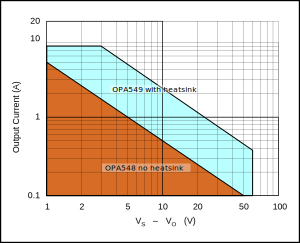
\includegraphics[width=0.8\textwidth]{OPA_SOAs/OPA_SOA}
	\caption{Safe Operating Area (SOA) for the OPA devices. $V_S$ and $V_O$ are the supply voltage and output voltage respectively. For the OPA549, this assumes the use of the heat-sink recommended. Diagram adapted from the OPA548 and OPA549 data-sheets. The OPA549 is not available with the 4 channel board option. }
	\label{fig:OPA_SOA}
\end{figure}

% subsection opa_choice (end)

\section{OPA gain} % (fold)
\label{sub:opa_gain}

The DAC outputs voltages ranging from \SI{0}{\volt} to \SI{2.5}{\volt}. These are amplified by the OPA opamps to reach the desired output voltages. The choice of gain resistors R12 to R19 set the gain of this amplification and therefore the maximum possible output voltage using the formula:

\begin{equation}
\label{eq:OPA_Gain}
G = \frac{Rx + Ry}{Rx} \implies
V_{max} = \frac{Rx + Ry}{Rx} \times \SI{2.5}{\volt}
\end{equation}

\textit{Default: \SI{100}{\kilo\ohm} and \SI{500}{\kilo\ohm}, gain = 6x, $V_{max} =\SI{15}{\volt}$}

\section{Instrumentation gain}

The input current sensing chips work by current through a gain resistor to match the current difference between the thermistor and set resistor they are measuring, as described in Section~\ref{sub:ina330_thermistor_amplifier}. The choice of resistors $R_{gain1}$ and $R_{gain2}$ therefore set the range of inputs that are available. 

For precise sensing near the setpoint, a large gain should be chosen. However, in order to make possible a wide range of inputs, a smaller gain is appropriate. If you choose to alter the default gains, you must ensure that both $R_{gain1}$ and $R_{gain2}$ are the same and their values are updated in {\tt Pins.h} (see Section~\ref{ssec:Pins}). 

\textit{Default: \RGain{} giving a \tempRange{} temperature sensing range}

\section{Setpoint resistors}
\label{sec:setpoint_resistors}

For applications that do not require extreme stability, it is possible to place the set resistor on the board in footprints $R_{prec1}$ and $R_{prec2}$. If this is done, the external precision resistor connections should not be made.

Although it is possible to lock to arbitrary resistance values, various advantages are gained by operating at the point where $R_{thermistor} = R_{set}$. In particular, operating at this point means that noise in the voltage reference or EMF noise from other sources will not affect the setpoint. Also, for small values of $V_{out}$ the device will increase the gain of the input stage of the ADC, allowing greater sensitivity. 

Again, for less demanding applications this is unnecessary: on-board precision resistors and digitally defined setpoints will provide sufficient resolution.

% \todo{Quantize resolution loss with on-board resistors}

\textit{Default: \RSet{} on-board resistors}

\section{Sensing series resistors}

Unfortunately, the INA330 instrumentation amplifiers struggle to drive even modest capacitive loads, such as that presented by \SI{30}{\cm} of BNC cable. For this reason a \SI{1}{\kilo\ohm} resistor is necessary in series with the thermistor and precision resistor to prevent bias voltage oscillations.

For the most demanding applications this series resistor can be removed and replaced with a piece of wire, reducing sensitivity to board temperature but necessitating short wires to the thermistor / set resistor. 

\textit{Default: \RSeries{} precision resistor}

\section{Pins.h}
\label{ssec:Pins}

Once customisation options have been chosen, the user must re-flash the device with a version of the source code reflecting these choices. To do this, the file \texttt{Pins.h} should be updated with the changes made and then the software should be compiled and uploaded using e.g. the Arduino IDE. Remember to temporarily re-enable flashing by using the vertical switch on the front panel. 

% section options_and_hardware_configuration (end)

\chapter{Initial setup} % (fold)
\label{sec:initial_setup}

The procedure for setting up a board is therefore as follows:

\begin{enumerate}
	\item \textit{Optional: Choose what configuration you require in accordance with Section~\ref{sec:options_and_hardware_configuration}, or accept the defaults.}
	\item \textit{Optional: If you chose to customize your board in the previous step, make these modifications now. }
	\item \textit{Optional: Open the {\tt Pins.h} file in the MC software folder. Edit it in accordance with your choices or leave it at defaults. (See the Doxygen documentation (Appendix~\ref{chap:full_doxygen_documentation}) for an in-depth description of each option)}

	\item Solder the OPA drivers you chose to the board if using the single channel board. The dual channel board comes pre-populated. 

	\item Using Atmel Studio and an AVRISP mkII programmer, connect to the ISCP header on the board and upload the Optiboot boot-loader file \path{./Code for Microcontroller/optiboot_xplained328p.hex}. This step only has to be performed once per microprocessor. 

	The board must be powered via the barrel-jack connector during this step. 
	\item Using the Arduino IDE, compile and upload the code to the device. After this is done, remember to re-enable flashing using the {\tt FLASH\_DISABLE} jumper. 
	
\end{enumerate}

After this process is complete, the device will appear over USB as a COM port. In order to test that everything went well, send the command {\tt *TST} (at baud rate \baudrate). If the response ``OK" is received, the software is installed correctly and communication between the microprocessor and the ADC is working. 

\todo{*TST not currently implemented}

% section initial_setup (end)

\chapter{Voltage Conversion Formulae} % (fold)
\label{sec:voltage_conversion_formulae}

The readings output by the device will be in volts, whereas usually the user will be interested in determining the resistance of a thermistor. For more details about how this voltage is produced, see Section~\ref{sub:ina330_thermistor_amplifier}. The voltage output $V_{out}$ is the voltage produced by the INA330 instrumentation amplifier according to its gain resistor $R_{gain1}$ or $R_{gain2}$. To convert this to a resistance, you must know the resistance of the set resistor (default $R_{set} = \RSet$), the excitation voltage ($V_{excite} = \SI{\VExcite}{\volt}$), the gain resistance ($R_{gain} = \RGain$) and the series resistance (default $R_{series} = \RSeries$). Use the following formulae:

\begin{equation}
\label{eq:volt_to_resistance}
R_{therm} = \left[ \frac{1}{R_{set} + R_{series}} - 
	\frac{V_{out}}{V_{excite} . R_{gain}} \right] ^ {-1}
	- R_{series}
\end{equation} 

or

\begin{equation}
\label{eq:resistance_to_voltage}
V_{out} = V_{excite} R_{gain} \left[ \frac{1}{R_{set} + R_{series}} - \frac{1}{R_{therm} + R_{series}} \right]
\end{equation} 

Thus, close to the set point, i.e. for small values of $V_{out}$, $V_{out}$ is linearly related to resistance. 

% section voltage_conversion_formulae (end)

\chapter{Hardware Design} % (fold)
\label{sec:hardware_design}

The board is designed to be rack-mounted with dimensions of $\SI{100}{\mm} \times \SI{80}{\mm}$. It is compatible with IEC 60297-3/-4 specs regarding dimensions and can fit front panels such as e.g. RS 258-2920. 

% This corresponds to half Eurocard format with an additional \SI{20}{\mm} added to provide space for the backplane connection. If this connection is not required it can be removed from the board (either at the printing stage or with a saw!) without impacting upon the rest of the board. \todo{Make Eurocard chopping possible}

\section{Isolation}

Since the error signals read by this board are at DC, much care was taken to avoid ground loops and crosstalk that could introduce bias. The ADC described in Section~\ref{sub:ads1262_analog_to_digital_converter} implements various filtering methods, but the board is also designed to prevent extraneous noise. 

The USB input interface is opto-isolated from the rest of the board, with power for the FTDI USB chip provided by the computer host. Also the entire analog section; incorporating the ADC, instrumentation amplifiers and input opamps; is isolated from the rest of the board and powered by a DC-DC converter. 

Although the output stages are not isolated from the rest of the board due to their high power requirements, care has been taken to manage high frequency digital return current in order to avoid signal crosstalk. The board has internal ground and power planes to reduce EMI and these both contain a bottleneck at the DAC: the point at which digital signals end and analog signals begin. This design is intended to keep digital return currents within the digital section of the board, avoiding pollution of the output stages. 

\begin{figure}[h!]
	\centering
	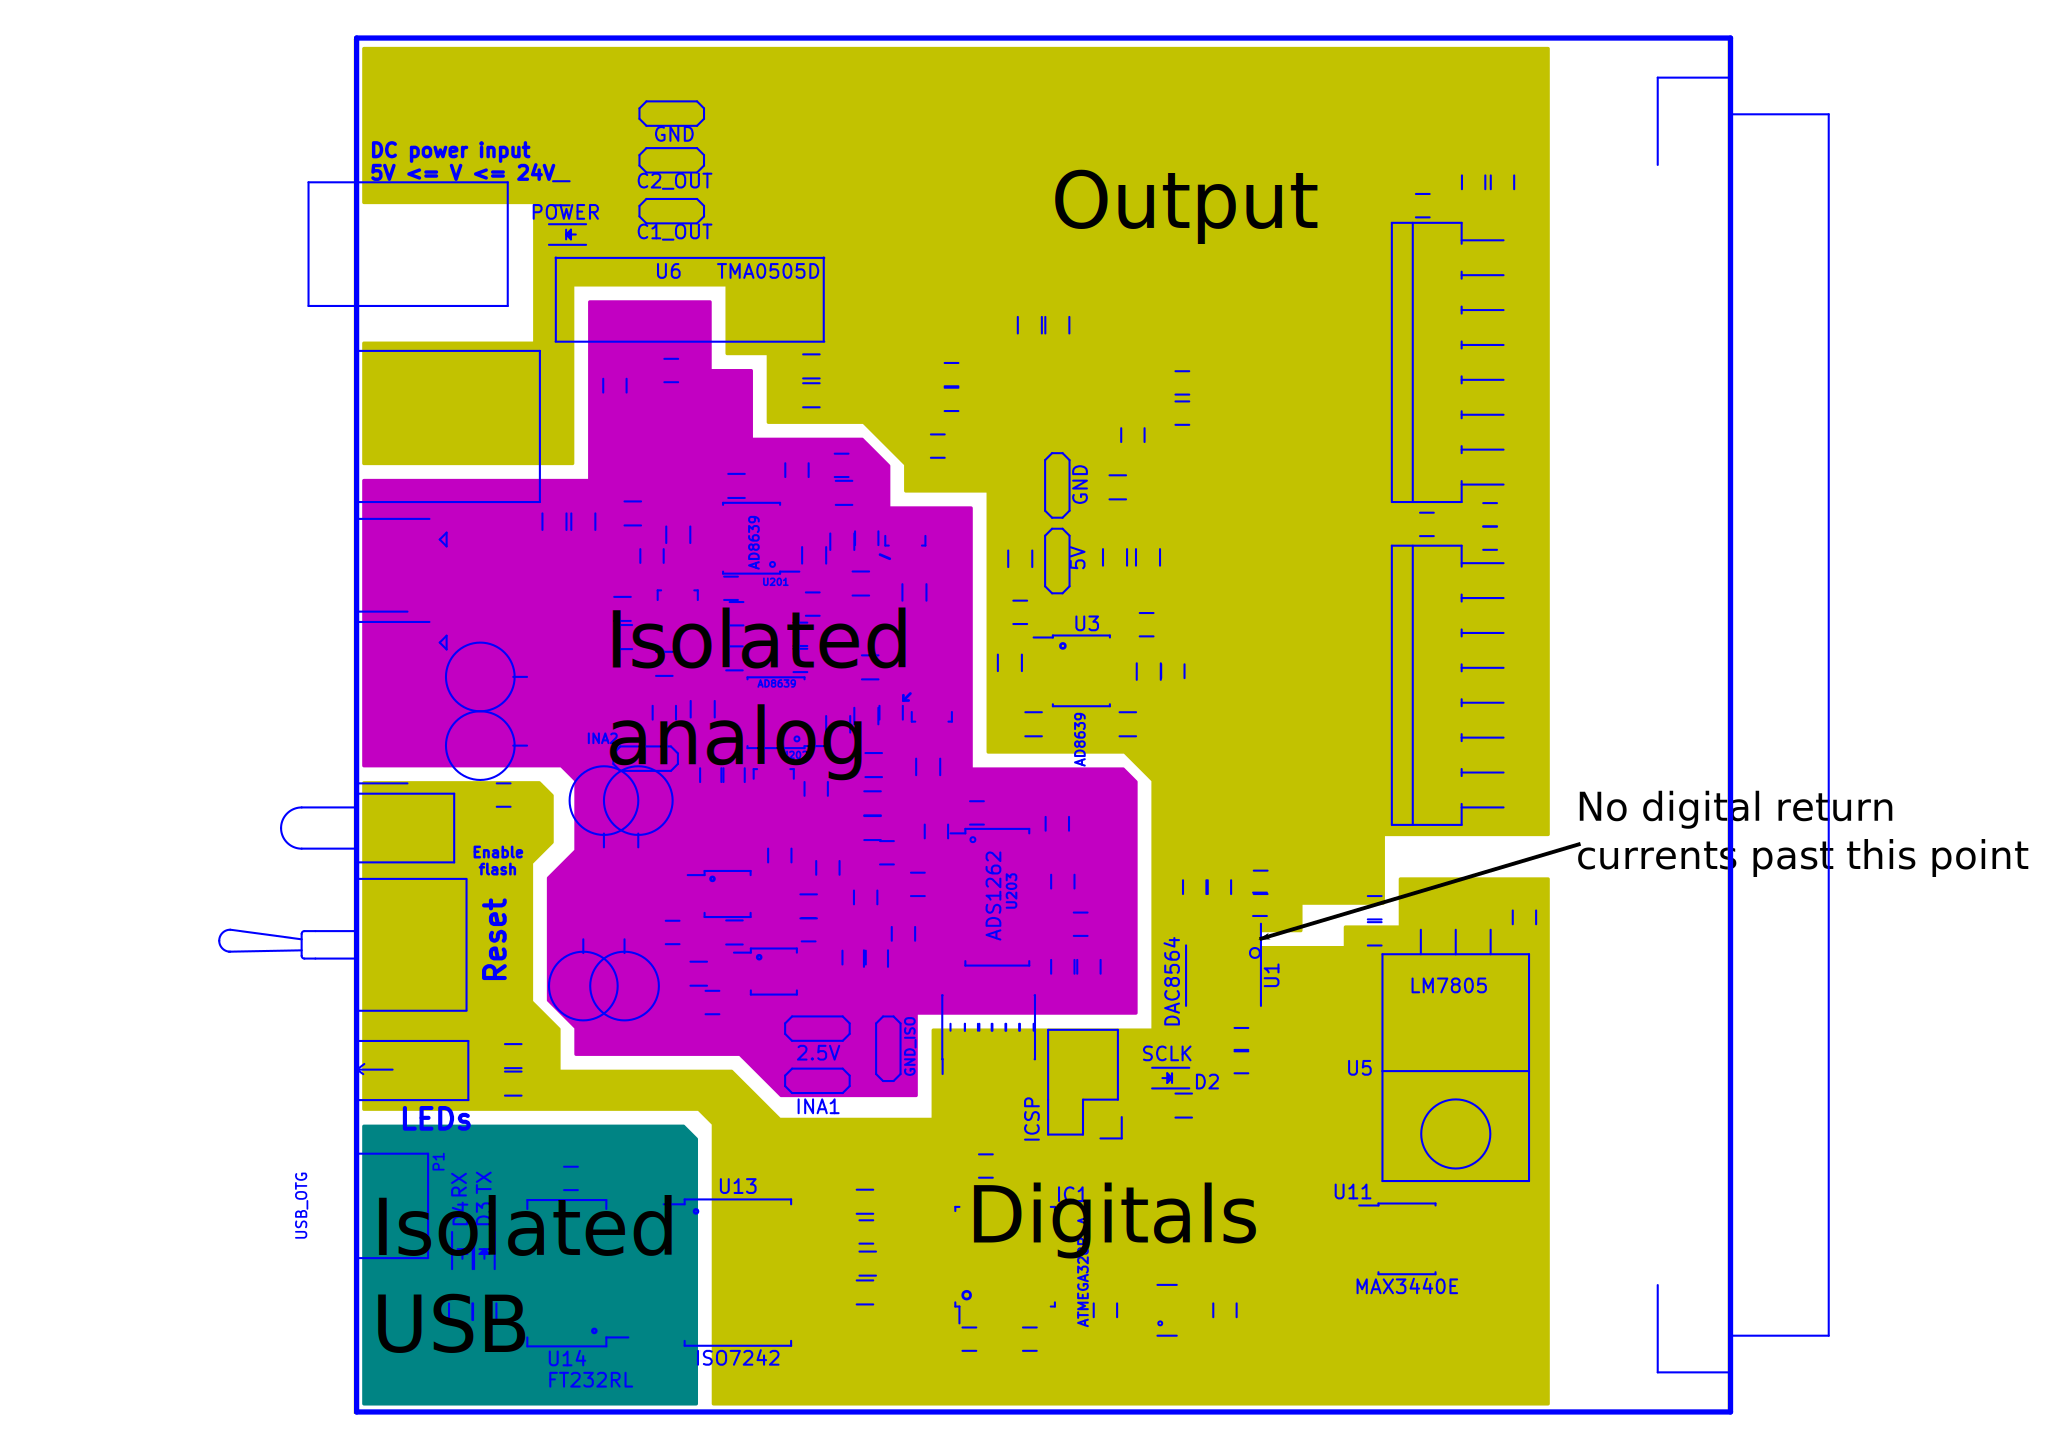
\includegraphics[width=\textwidth]{BoardIsolation/BoardIsolation}
	\caption{Segmentation of the 2 channel board for isolation and ground loop considerations. 4 channel board is similar}
	\label{fig:isolation}
\end{figure}

\section{ADS1262 - Analog to Digital Converter} % (fold)
\label{sub:ads1262_analog_to_digital_converter}

The ADS1262 is a nominal 32-bit ADC produced by Texas Instruments. During a temperature reading it is configured to use a two stage digital filter. The first order provides a fixed 5th order sinc filter. The second stage is a programmable order sinc filter, set to 4th order. These two together result in an \SI{0.58}{\Hz} \SI{-3}{\dB} bandwidth, with poles at \SI{50}{\Hz}. On top of this, a simple analog external RC low-pass filter prevents aliasing. 

The ADS1262 has inherently low input offset bias however, to combat any residual bias, every measurement is taken twice with the input signal paths swapped over via the internal analog MUX. 

The IC also contains an optional Programmable Gain Amplifier (PGA) stage. The micro controller monitors the signals it reads and, if it detects several measurements in a row that would have benefited from increased gain, it automatically boosts the gain stage to increase sensitivity further. If the signal later becomes too large for the gain selected this is also automatically detected and corrected by the micro controller. 

Because of this re-sampling and filtering, a single measurement can take up to \SI{5}{\second} to complete. Programs that interface with the temperature controller should therefore be aware that commands such as {\tt ERRO? 1t} can take up to \SI{5}{\second} and should take appropriate steps to avoid timeout. The Labview interface handles this automatically. 

\begin{figure}[h!]
	\centering
	\includegraphics[width=\textwidth]{ADS_diagram}
	\caption{Flow diagram of the ADS1262. Reference: ADS1262 datasheet by Texas Instruments}
	\label{fig:ADS_Flow}
\end{figure}

% subsection ads1262_analog_to_digital_converter (end)

\section{INA330 - Thermistor Amplifier} % (fold)
\label{sub:ina330_thermistor_amplifier}

\begin{figure}[tb]
	\centering
	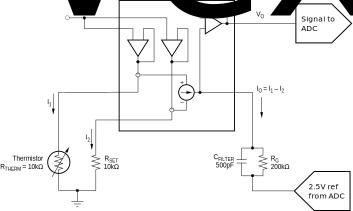
\includegraphics[width=0.8\textwidth]{INA_Flow/INA_Flow}
	\caption{Flow diagram of the INA330. The \SI{2.5}{\volt} reference comes from the ADC and the output voltage is refereed to this reference. The \SI{\VExcite}{\volt} excitation reference is derived from the \SI{2.5}{\volt} reference ratiomatically for maximum common-mode rejection. Diagram adapted from INA330 datasheet by Texas Instruments.}
	\label{fig:INA_Flow}
\end{figure}

The thermistor / setpoint precision resistor comparison is done by an INA330 chip. These chips take a reference voltage, \SI{\VExcite}{\volt} on this board, ratiomatically derived from the stable \SI{2.5}{\volt} reference of the ADS1262. This is buffered and used to drive both the thermistor and the resistor. The current difference between these two arms is then forced through a gain resistor, $R_{gain1}$ or $R_{gain2}$ (by default \RGain), amplifying it with respect to the \SI{2.5}{\volt} reference. This signal is then read by the ADC and compared to the \SI{2.5}{\volt} reference in differential mode. 

Figure~\ref{fig:INA_Flow} shows a schematic of the INA's operation. 
For a resistance to voltage conversion formula use Equation~\ref{eq:volt_to_resistance}.

% subsection ina330_thermistor_amplifier (end)

\section{OPA548/9 - Output Amplifiers} % (fold)
\label{sub:opa548_9_output_amplifiers}

The final output to the plant is handled by an OPA548. These amplify the $\SI{0}{\volt} \rightarrow \SI{2.5}{\volt}$ signal produced by the DAC to the voltage required by the user, set by gain resistors as described in Section~\ref{sub:opa_gain}.

% subsection opa548_9_output_amplifiers (end)

\section{DAC8564 - Digital to Analog Converter} % (fold)
\label{sub:dac8564_digital_to_analog_converter}

The production of the analog signal is done by the DAC8564: a 16-bit digital to analog converter, referenced to its own internal \SI{2.5}{\volt} reference. 

Its output ranges from \SI{0}{\volt} to \SI{2.5}{\volt}. This signal is then either amplified by the OPAs to become the output level, or doubled by a AD8639 auto-zeroing opamp to control the current limiting feature of the OPAs. 

% subsection dac8564_digital_to_analog_converter (end)

\section{ATMega328p - The micro controller} % (fold)
\label{sub:atmega328p_the_micro_controller}

The brain of the device is an ATMega328p MC. This is the same processor that is found on the Arduino Uno or Nano, and the board is configured (instructions in Section~\ref{sec:initial_setup}) to appear as an Arduino Nano to the computer. However, by breaking the Arduino into pieces several advantages are gained including reduced board space and the option to add on-board isolation to the USB interface. 

The ATMega is clocked from a \SI{16}{\MHz} full-swing crystal. When the board is assembled for the first time the ATMega's flash memory will be blank and the device with not be programmable over the usual USB interface. For the first time only, programming must be done by the ISCP header provided, as described in Section~\ref{sec:initial_setup}. 

% subsection atmega328p_the_micro_controller (end)

% \section{Backplane} % (fold)
% \label{sub:hardware_backplane}

% The board is also equipped with an optional DIN41612 backplane connector, RS number 252-210. If used, the board draws its power from the 24V rail of the backplane and must not be powered from the front panel. 

% Connecting the backplane also enables RS485 communication. Although the software for this has not, at the time of writing, been developed, this hardware layer in combination with the Modbus protocol should enable easy, collision-free control of an entire rack of devices using a single USB connection. 

% subsection backplane (end)

\section{RS485} % (fold)
\label{sec:rs485}

The board is equipped with a 4 pin Molex PicoBlade 53048-0410 connector that enables RS485 communications. This is currently unimplemented, but will allow for control of up to 255 RS485 boards from a single USB connection. 

% section rs485 (end)

% section hardware_design (end)

\chapter{Software Structure} % (fold)
\label{sec:software_structure}

The code running on the micro-controller is written in C++. The ATMega328 is set up to appear the same as an Arduino Nano: it is therefore possible to compile and upload the code using the usual Arduino IDE. Note that re-flashing like this this requires two things: a) the {\tt FLASH\_DISABLE} switch should be set correctly (see Section~\ref{sub:switches}) and b) the boot-loader must have been installed using the ISCP header (see Section~\ref{sec:initial_setup}). 

The code-base makes considerable use of the object-orientated programming style. While this can appear daunting at first, in the long run it simplifies modifications and results in more compartmentalized code that is easier to understand. This overview and the more in-depth Doxygen documentation both assume some familiarity with concepts such as virtualisation, inheritance, abstraction and polymorphism.

There are very many online and offline resources that can give you an overview of these ranging from 1 page to multiple-volume books. For a quick starting point, try \url{https://www.cs.bu.edu/teaching/cpp/inheritance/intro/} and \url{https://www.cs.bu.edu/teaching/cpp/polymorphism/intro/}. 

\section{Doxygen} % (fold)
\label{sub:doxygen}

The code is thoroughly commented throughout to aid comprehension. These comments have been written to comply with the requirements of the documentation program Doxygen \url{http://www.stack.nl/~dimitri/doxygen/}. It is therefore simple to compile all these comments into a manual by installing the Doxygen program on your computer, launching the wizard, selecting the {\tt Doxyfile} file in the temperature controller's source code and running the wizard. This will produce a neatly linked set of HTML files that can be opened in any browser. It will also produce \LaTeX{} output, the result of which is appended to this document in Appendix~\ref{chap:full_doxygen_documentation}. 

The Doxygen output is detailed and should be considered the authority if modification to the code is required, but this section provides an overview of the code structure. 

% subsection doxygen (end)

\section{Code Overview} % (fold)
\label{sub:code_overview}

As per usual object-orientated design, the jobs performed by the temperature controller are split between objects. Two of the most important are ErrorChannels and CtrlChannels. These classes manage interactions with the world. They are abstract classes, and provide a template of functions which must be fulfilled by their derived classes. 

For instance, CtrlChannels have a method setCtrl() which sets the output voltage available at the OPA. This method takes a double as a parameter, the new control level, which adheres to a convention used throughout the code: all error readings or control outputs are given as a number between -1 and +1 where -1 corresponds to the lowest possible level and +1 corresponds to the highest. 

A specialisation of CtrlChannel is V4\_OPA\_OutputChannel. This overrides the ``pure virtual'' methods in CtrlChannel and writes a voltage to the output channel it manages. On initialisation this object is assigned to one of the OPAs. A value of for output -1 would correspond to 0V, a value of +1 would be {\tt +MAX\_VOLTAGE} V. 

A different specialisation of CtrlChannel is V4\_OPA\_OutputChannelBipolar. This object also performs output, but rather than outputting a voltage on a single OPA, it uses 2 OPAs at the same time in order to output a bipolar differential level. 

ErrorChannels have similar functionality but are used for input instead of output. However, since taking a reading can take several seconds (see Section~\ref{sub:ads1262_analog_to_digital_converter}) there is a bit more structure involved. Readings are initiated with startReading(). Before this happens, the calling code should check that no reading is already in progress by calling globalReadInProgress(). Once a reading has been started, its progress can be checked by calling readingReady() and then its result can be output using getReading(). 

Other important objects in the code are:

\begin{description}
	\item[Controllers]  Contain references to an ErrorChannel, a CtrlChannel and an Algorithm. Every time doLoop() is called, attempt to take a reading from the ErrorChannel, process it with the Algorithm and output it with the CtrlChannel. 

	\item[Algorithms] An abstract class that defines an object responsible for processing an input error signal and returning the new control level. This object should contain information about the set-point and any limits applied. An example implementation is PIDAlgorithm. 

	\item[CommandHandler] An independent object that can be included as an Arduino library in any project. This object manages the input and parsing of serial commands. It uses a hashing algorithm to minimize memory consumption and assigns all memory on the stack to avoid fragmentation. It is responsible for calling the appropriate function when a command is issued. See its own Doxygen documentation for much more detail. 
\end{description}

A typical cycle in the code looks like this:

\begin{enumerate}
	
	\item Check CommandHandler for new commands and execute them if present. 
	\item For all Controllers, see if a lock is in progress
	\item If so:
	\begin{itemize}
	 	\item If an ADC reading is in progress do nothing. 
	 	\item If no reading is in progress, start one. 
	 	\item If an ADC reading for this channel is complete, get the result and move to step 4. 
	 \end{itemize} 
	\item Feed the result of the reading into the contained Algorithm
	\item Get the new control level back from the Algorithm and pass this to a CtrlChannel for output. 

\end{enumerate}

% subsection code_overview (end)
% section software_structure (end)

\clearpage
\begin{appendices}

% \chapter{Todo list} % (fold)
% \label{sec:todo_list}

% % Hack to get todonotes to work with amsart
% \makeatletter
% \providecommand\@dotsep{5}
% \makeatother

% \listoftodos\relax

% section todo_list (end)

% \chapter{Known bugs} % (fold)
% \label{sec:known_bugs}

% section known_bugs (end)

% \chapter{Git} % (fold)
% \label{sec:git}

% \todo{Write git appendix}

% section git (end)

% \clearpage
% \chapter{What is Object Oriented Programming?} % (fold)
% \label{sec:the_object_paradigm}

% \textit{
% The following essay was written by Andrew Hardwick and released under the GPL license at \url{http://duramecho.com/ComputerInformation/WhatIsObjectOrientedProgramming.html}. This is a verbatim copy.
% It is intended as a quick introduction to the principles and benefits of Object-Orientated Programming (OOP). The target reader will have familiarity with programming concepts such as methods, variables, arrays but needs no knowledge of OOP. 
% }

% \section{Firstly: Don't Panic!}

% Object Oriented Programming (called `OOP' for short) is promoted as a radical, difficult to comprehend \& even frightening way of programming that vital to know about. Is this true? No.

% Object Oriented Programming is not very radical or very difficult compared to conventional programming. When one looks under the ideology and sees what is actually there, one finds there is not really much different at all!

% The reason for it seeming so difficult is that introductions to OOP are normally given by the follow types of people who are not ideal for teaching the basics:

% \begin{description}
% 	\item[OOP Zealots] These advocate OOP in seminars \& articles with great enthusiasm but leave the audience with little understanding of what OOP actually is, just a feeling that it is revolutionary \& complicated. The dogmatic fervour scares people off.

% 	\item[Computer Scientists] These marvel in lectures about the structures and relationships that an object oriented approach can bring and draw lots of rectangles, lozenges or clouds joined by lines This is rather pointless as it is all fairly obvious to the mathematically minded in the audience and is all totally incomprehensible to the rest. The boredom puts people off.

% 	\item[Programmers] These helpfully give the details of how to do particular things in particular OOP languages in web pages \& books but miss out the basic introductory explanations. The detail puts people off.
% 	\item[Incompetents] Unfortunately there are some of these. I've even come across a lecturer from a London university who was paid to teach us OOP but could not answer the first trivial question when challenged to explain the rhetoric. The confusion puts people off.
% \end{description}

% In the following article I will try to explain what OOP is and why it is used but without the customary hype, irrelevant extras \& detail (and, hopefully, without the incompetence). I am assuming the reader is familiar with the fundamental concepts of normal programming such as a program being made of `commands' which tell the computer do things, `variables' to store data in and the idea of grouping a set of commands together in `functions' (or `subroutines' which are virtually the same) which can be called as needed from different parts of a program. However, the ability to write programs is not required and I won't be giving the detailed syntax for any particular OOP language. If you want that then there are a surfeit of books \& web pages to choose from already.

% \section{What Object Oriented Programming is}

% Firstly, some background. A conventional (`procedural') program consists of a sequence of commands. The commands can do input, output, manipulate data and control the order in which the commands are carried out. So as not to have to duplicate commands in different places in a program where same action needs to be performed, a set of commands can be combined into a `function' or `subroutine' which acts like a new command. This same set of commands can then be called from different places in the program. As well as substantially reducing the length of programs, this can make the structure neater by encapsulating the commands which, together, perform some particular operation in one place. The rest of the program need not be concerned about the details of what commands make up the function and just treat it as something which does that operation. This neatness is not merely an aesthetic feature but a great aid to making programs quicker to write, easier to debug, more reliable \& more reusable.

% Splitting a program into functions makes programming quicker not only because different programmers may be able to work on separate functions at the same time but, crucially, it breaks down a huge task which would be difficult for a human to store in mind as one piece into smaller units more suited human memory. It makes debugging easier because it localises the effect of a single bug so it is easier to track down and, when bugs have been eliminated from a function, one need not waste time rechecking it when debugging other parts of the program. To aid this, it is normal to have the variables a function uses internally hidden from the rest of the program, unless there is a special necessity to reveal them. This ensures that any problem related to such a `local' variable can be traced to function which needs correcting. This also makes the program more reliable because, once a function is working, it should stay working as more of the program is built up. Other parts of the program cannot disrupt those hidden variables \& commands inside the function. The splitting also, of course, makes subsequent programs quicker to write as whole functions can be reused from earlier programs and even stored in libraries for use by any future program. The generic term for this is approach of breaking a big solution into small pieces whose internal workings are not of concern to other pieces is `modular'.

% Enough about functions. Now for variables. In many computer languages, a programmer can define a compound variable type in addition to those which are ready made in a language. For example if a particular language has variable types for names \& dates, a type for storing birth records could be made by combining two name type variables, for the family name and given names, with a date type variable, for the date of birth. These combined variables are called different things in different languages including `structures' (C), `clusters' (LabView) \& even just `types' (Fortran). Combined variable types can be useful. For example, instead of having to work on and pass around three variables together whenever a birth record is used, a single variable of this combine type could be thus be used. Commands \& functions which don't need to use all the member variables of a combined variable need not be concerned they are there. One can even copy a combined variable in one command, rather than one command for each member variable, without knowing or caring what all the member variables are. This is applying a modular approach to collections of variables as functions were for collections of commands.

% That was around for decades then someone then came up with the idea of including functions as well as variables in those combined variable types. Combined variable types could then have member functions as well as member variables. These functions are only really in the program once (it would be very inefficient otherwise) because they are written into the variable type specification not the individual variables of that type themselves. However, they act as if they were duplicated in each variable of that combined variable type because they, by default, act on the member variables of the particular variable of the variable they called with. For example one could have included a member function to calculate a person's age into that birth record combined variable type. When a particular variable of that type, storing a particular given name, family name \& date of birth, has its age calculating member function called, the function will automatically use the member variables of that particular variable, not the generic variable type, to calculate an age. This can be quite handy because it neatly bundles data \& the functions which act on it together. It can also aid conceptualising a program because, in calling a member function, one is effectively telling the data what to do to itself which is, in some situations, closer to reality than giving the data to a command to process.

% Now you have understood that, we can go onto Object Orientated Programming at last. Correction: if you have understood then you have understood Object Oriented Programming! That idea in the preceding paragraph of putting functions into combined variable types is Object Oriented Programming! Does it not sound dramatic enough? Okay, lets put some hype in: rename 'member functions' to `methods'; rename 'combined variable types' to `classes'; and rename 'variables of combined types' to `objects'. That's all it is!

% \section{A Few Little Extras}

% There are few useful extras which normally come with OOP. They can mostly exist in procedural programming languages as well so they are not necessarily OOP features but they are ubiquitous in OOP languages so I suppose I ought to mention them. You can skip this section if it is too detailed.

% \begin{description}
% 	\item[Data hiding] Just like functions can have local variables not visible to the rest of the program, so can objects. This is for storing data that is not revealed or set directly but only via methods (member functions). For example a birth record object could store the year, month \& day of birth in separate member variables and only combine them when asked for date of birth by a method call. Some OOP advocates even recommend that all member variables are hidden and only accessed via methods but that is sometimes excessive.
% 	\item[Automatic initialisation] A class can have a method (called a `constructor') which is automatically called whenever a new object of that class comes into being. This like having a default value for a variable type that a variable is initialized to when it is created prior to being set. However, as objects have member functions (methods) as well as member variables, this has been generalised into a method call that can do a lot more than just set a default value. There is a corresponding method (called a `destructor') which is called when an object is disposed of and is typically used for clearing up.
% 	\item[Same name, different function] Different functions can have the same name provided they are distinguished by their parameter types. This is useful in procedural languages but is almost vital in OOP languages because classes may come with functions that take objects of the class as parameters (as well as member functions embedded in the class) and it likely that there will be a duplication of popular function names between classes from different programmers. In OOP, this ability to have multiple functions with the same name is called `overloading'.
% 	\item[Derived classes] If one requires a class which like a class one already has but requires extra features then one can derive a class from an existing class. The derived class has all the externally visible methods \& member variables the base class it was derived from had (and, optionally, some of the hidden ones) plus whatever extras are put in. For example one could derive a class from birth record class that also a member variable for time of birth or a method for combining the family \& given name into a full name. Besides aiding reuse of program parts, it is possible to have different derived classes from the same base class for slightly different situations. For example British \& Chinese versions of the previous example could be made where the British one calculates a full name by appending the family name to the given name whereas the Chinese one joins them the other way around. A nice feature of this is that objects of both types could then be stored and processed the same (thereby saving programming) and yet perform differently when the full name method is called. In OOP, this ability to have the same function perform different actions depending on the derived class is called `polymorphism'.
% \end{description}

% \section{Why it can be Good Thing}

% OOP is good for the same reasons that other modular programming schemes are: aesthetic neatness, quick writing, eased debugging, improved reliability \& increased reusability in large programs.

% In addition, an object based structure naturally fits certain common uses of computer programs including graphical user interfaces (with buttons, windows, scroll bars as objects) and databases (records as objects).

% Of course, all this the modular structuring can be done with a classical `procedural' language (indeed the OOP C++ language was originally made a collection of `search \& replace' operations that converted C++ programs to the procedural C language!) but looks cleaner in OOP because OOP was designed for this structuring. And OOP is fashionable!!

% \section{Why it can be a Bad Thing}

% There are drawbacks to OOP as well. It is not the best thing to use in all circumstances. Don't fall into the trap of using for ideological reasons when it is not the most suitable method for a particular task (and similarly don't dogmatically stick to a single programming language, pick the more suitable one for each job).

% For a start, it should be obvious that OOP, or any such heavy programming method, is probably not ideal for doing small quickly-written one-off programs where the time taken to define a class structure is more than the time you will save by having it neatly modular. Of course, one can use an OOP language for short programs, it is just that structuring your own programs in an OOP fashion in addition to using the language's in-built own objects would be inefficient. I don't know what the cross-over point is but I guess it is several hundred lines of program for myself, although I would probably do modular structuring into functions at well below a hundred lines.

% Neither is it suitable for very low power computers such as the microcontrollers embedded in consumer products which often have only less than a kilobyte of memory to fit the program into (compared to gigabytes on a office PC) and only a few bytes (compared to megabytes) to store variables in.

% There are also some jobs which are naturally ``do this ... then this ... then this ... then this ..." tasks in which case programming it procedurally could well be neater and easier than doing it object oriented. I've found this for simple one-task programs that control mechanical devices or batch process files. They typically read in the parameters, read in data from files, apply a series a manipulations to the data \& parameters and output to electronic hardware or to a file in that order. Sometimes they don't even have conditionals or loops. Object orientation would be an ill-fitting arrangement for these programs. (An interesting aside: often such small programs are called in turn by other small programs and a collection of such programs naturally builds up into an effectively object oriented system, where the little programs act as classes, without any planned intention for them to be so.)

% The most serious drawback is one common to all neatly structured modular programming: the division into modules really needs to be decided in advance of programming. In an ideal programming situation this would be the case but, in reality, customers who don't understand programming often change the requirements drastically after programming has been started (or even finished!). Often spec's are changed in a way that looks small from the outside but which mean that objects which were built to act totally independently of each other are changed so that they need to control eachother directly. The program alterations are then either a time-consuming restructuring of much of the program or messy ad-hoc direct links which wreck the modularity. For example, if a customer asked for a simple product database in which records are only ever set once \& recalled one at a time for reading, then the obvious class structure would be one of a records class for storing the product data and a database class consisting of an array of those customer records objects along with a method to add a new record object and search method to returns a copy of a requested record for reading. If the customer then demands that a product record should link to related products with the links changeable from the display terminal, then the structuring will be serious. Not only will it need that extra variable added to the record class (easy) but record objects will need to link to other record objects which was previously only via the database object (disrupts the neat modular structure), the database will need to pass around the original record object instead of a copy so it can be altered (lots of changes needed in different places in the program) and a contention-resolution system will be needed to prevent the records now being altered from different parts of the program simultaneously (a difficult and time consuming programming task). The only solution I know of for this is to warn customers that such spec' changing is like asking for different foundations in a house after the walls are built and get them to contractually agree to pay for such alterations they request but customers don't like that.

% \section{The Real Reasons that it is so Popular in C/C++!}

% The rest of this article was not language specific but one major misconception needs to be cleared up with the language`'C++'.

% OOP is most commonly advocated for `C++'. In part this advocacy is just because `C++' is the procedural language `C' with OOP added in later so they make a nice pair of languages to compare \& contrast unlike, for example, `Java' which was OOP from its first creation. However this does not explain the fanatical enthusiasm with which C++ was welcomed. Was the explanation that OOP was so much better than procedural programming? No. It was simply that there were some very useful things absent from the original C language that were either rectified in C++ or could be bodged up with OOP tricks:

% \begin{description}
% 	\item[Strings \& arrays] Almost amazingly, C does not really have variables of string or array type. Instead strings \& arrays have to be cumbersomely bodged in using pointers to general-purpose chunks of memory with the programmer having to maintain separate records of where they are \& how long they are and resort to tedious explicit memory cell copying operations to duplicate them or change their lengths. Although C++ does not come with strings or arrays either, one can write classes which encapsulate the memory manipulation routines and, at last, use instances of them as if they were intrinsic string \& array variables without further hassle. (Other than the hassle of there being many different string \& array classes and each product's library seems to use different ones which need interconversion! Even I have written my own ones after finding the ones that came with the MS C++ compiler were not fast, easy or reliable enough for my requirements.)
% 	\item[Memory deallocation] Despite C programming needing so much direct memory manipulation, it does not automatically free up memory when it is no longer needed like Perl \& Java do. Therefore the programmer must write their programs so that they tediously keep track of all memory that has been allocated by request and explicitly free it up when no longer needed. This is especially tedious where there are many ways a function can exit (such as after testing for different errors) and each one must have commands to free up the same memory. If this is not done then the computer runs out of memory as more \& more of it is left reserved but not actually in use (a situation so common that it has the been given the name of a ``memory leak"!). Although C++ still has this problem, it is slightly less hassle as one can create classes for the variables which need memory allocation, perform the allocation in the class's constructor \& free it up in its destructor so one only needs to program the freeing up in once instead of everywhere such a variable might cease being used.
% 	\item[Function overloading] It is annoying in C that if one wants to write a function that can process more than one type of variable then one has to give the functions different names and type the correct name for the data type when using it. For example one has to use `abs()' to calculate to the absolute (unsigned) value of an integer but `fabs()' to do the same thing for a floating point number. The compiler should be able to distinguish these itself from the type of parameter. In C++ it can. This is not a specifically OOP feature though.
% 	\item[Unspecified variable type] C likes to know what type its variables are even when the specific features of that type are irrelevant. This annoying when wants to store a collection of variables of different types in an array or write a program that will not need reprogramming when new types are added. The normal solution is to have duplicate commands for the different types or a messy ``void pointer" fudge. With OOP one can derive all ones variable types on one base class (even if that base class does absolutely nothing!) and treat them all as being of that type.
% 	\item[Localised namespaces] When writing a big program, it is difficult to ensure that names of functions are not duplicated in different files. This is especially a problem for little functions which need not be visible to other modules, just for use internally. A name like 'IncreaseCount()' could easily be accidentally duplicated. A common solution was to start each function name with the name of the file or module which it was in but that was messy, increased typing \& actually broke the official C spec' (which stated compilers could ignore all but the first 6 characters of function names). In C++ there is a neater bodge-up: bunging all the functions from one file or module in a class, even if that class does not have any variables, neatly localises the function names. Once more, this is need not have required OOP; for example, in the Perl language one can specify anything to be only locally visible (indeed adding OOP features to Perl required almost no changes to the language, essentially just an alternative syntax which called such localised regions classes!).
% 	\item[//] The most commonly used C++ feature, which is now used ubiquitously in programs which otherwise use only pure C commands, is the `//' command which merely means ``ignore everything else on this line"! It is quicker to type than the original C comment markers '/*...*/' which needed one to mark both ends of the stuff to ignore.
% \end{description}

% The reason for these deficiencies in C is because C was designed for low level fast programs on low power computers not for database \& graphical user interface programs on the far more powerful computers available at present. It is C++'s adaptation of C towards this changed role which gives it its popularity not so much its OOP nature.

% \section{Summary}

% Object Oriented Programming is not as different from normal procedural programming as is made out by its advocates and is not as difficult to understand as their proselytising implies. It is useful in making big modular programs but such programs should have been structured very similar to an OOP structure anyway. It can be more hassle than it is worth for short \& quick programs. The enthusiasm for C++ in particular is mainly because it adds in some important basic features that were missing from C.

% % section the_object_paradigm (end)

% section overview (end)
\chapter{Available Commands} % (fold)
\label{chap:available_commands}

The commands recognised by the controller are defined in the file \path{./Code_for_microcontroller/YbTempCtrl/CommandDefinitions.h} and the Doxygen documentation (Appendix~\ref{chap:full_doxygen_documentation}) for this file contains a complete list of them. 

This documentation is reproduced here for convenience. The following is automatically generated from the code's markup, so please excuse any odd formatting. All parameters should be separated by spaces. All commands must be followed by a newline (ASCII 10) character. 

\input{../Code_for_microcontroller/YbTempCtrl/doc/latex/_command_definitions_8h.tex}

\chapter{Full Doxygen documentation} % (fold)
\label{chap:full_doxygen_documentation}

The following pages are the full documentation of the code, produced automatically by Doxygen. Doxygen is a code commenting system that allows you to write structured comments throughout your code which can later be extracted into a code reference.

To get the latest version of this reference, incorperating any changes, you need to install Doxygen, run the Doxywizard, load the file \path{./Code_for_microcontroller/YbTempCtrl/Doxyfile} and click ``Run doxygen''. This will produce HTML and \LaTeX{} output. 

It will also generate a file called \path{make.bat} in \path{./Code_for_microcontroller/YbTempCtrl/doc/latex/make.bat}. Execute this file to produce the updated \LaTeX{} code reference. To incorperate this into the manual you are currently reading, just recompile the latex from \path{./Manual/TemperatureControllerManual.tex}. 

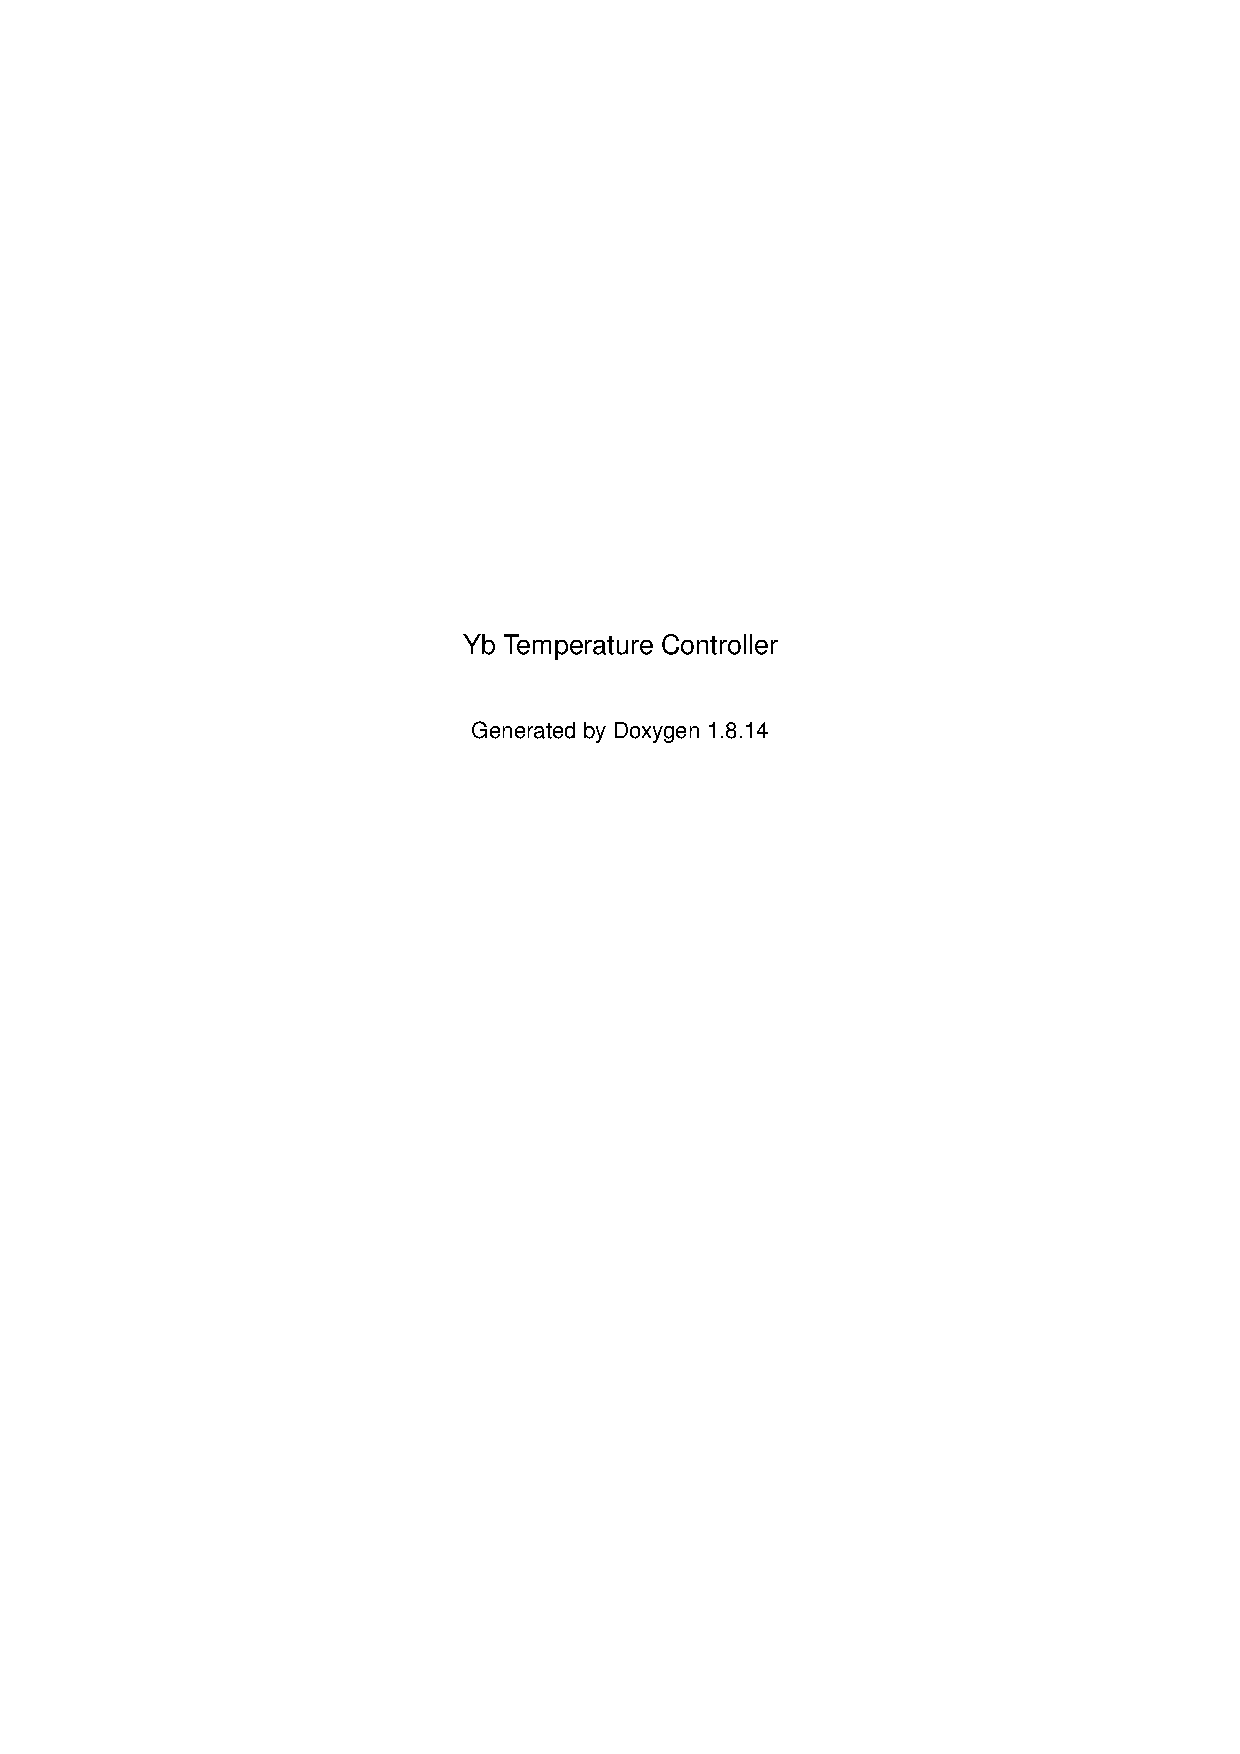
\includepdf[pages={-}]{../Code_for_microcontroller/YbTempCtrl/doc/latex/refman.pdf}

% chapter full_code_documentation (end)

\end{appendices}

\end{document}  